\subsection{Högn und der Nationalsozialismus}

\label{bkm:Ref99597687}\hypertarget{RefHeadingToc100333734}{}\label{bkm:Ref99597697}\label{bkm:Ref99597694}Aus
den Jahren 1936 und 1937 sind Dokumente erhalten, in denen August Högn
in der Funktion des Beauftragten für {\textquotedbl}Schutz des
Volksguts{\textquotedbl}, \footnote{Dokument Nr. 162, Brief von Albert
Schroll, Gemeindesekretär an August Högn, 21.1.1937}
Untergruppenführers \footnote{Dokument Nr. 128, Einteilung der
Gemeindegruppe Viechtach, 5.7.1937} und
Gemeindegruppenführers \footnote{Dokument Nr. 130, Brief von
Gemeindegruppenführer August Högn an alle Block- u. Hauswarte,
23.10.1936} hervortritt. Mit „Schutz des Volksguts“ wurden zur NS-Zeit
Metallsammlungen bezeichnet, an die sich auch die Schulen
beteiligten. \footnote{Interview Nr. 17, Max Holler, 26.8.2004, Absatz
16} Aus einem Dokument geht hervor, dass Högn als Führer der
Untergruppe Ruhmannsfelden der Gemeindegruppe Viechtach vier Blockwarte
unter sich hatte. \footnote{Dokument Nr. 128, Einteilung der
Gemeindegruppe Viechtach, 5.7.1937} In einem anderen Dokument
unterzeichnete der Gemeindegruppenführer Högn, wohl synonym gebraucht
zu Untergruppenführer, eine Einladung an alle Haus- und Blockwarte zur
Schulung im Luftschutz. Aufgrund der unvorstellbaren Verbrechen des
NS-Regimes sind Fragen nach der Zusammenarbeit des Einzelnen mit dem
damaligen Regime natürlich auch 60 Jahre nach Ende des 2. Weltkrieges
zu Recht von großer Brisanz. Doch sei vor voreiliger Vorverurteilungen
gewarnt, denn die wenigsten heute in der demokratischen Bundesrepublik
Deutschland lebenden Menschen haben diese totalitäre Diktatur mit ihren
indoktrinären Mechanismen bewusst miterlebt. Auch anhand einer noch so
drückend erscheinenden Beweislast, kann man letztlich doch nicht in
jemanden „hineinschauen“ und feststellen, ob stark das Engagement des
Einzelnen für den NS-Staat tatsächlich aus innerster Überzeugung
erfolgte. Anhand der im Folgenden geschilderten Fakten soll sich
deshalb jeder für sich selbst ein Bild von August Högn Einstellungs zur
Politik im 3. Reich machen.

Die Bewunderung, die Högn für seinen Schwiegersohn Dr. Karl
Schlumprecht, besonders für dessen politische Karriere zeigte\footnote{
Interview Nr. 20, Gertraud von Molo, 23.11.2004, Absatz 34} und das
gute Verhältnis zu ihm, \footnote{Interview Nr. 2, Barbara Essigmann,
27.12.2002, Absatz 66} sind Indizien dafür, dass Högn die Ideologie des
Nationalsozialismus nicht von Grund auf ablehnt hat. Dr. Karl
Schlumprecht war nach der Machtübernahme der NSDAP erster
nationalsozialistischer Oberbürgermeister von Bayreuth bis April
1937. \footnote{http://www.bnbt.de/\~{}tr1035/bt/wer/index.htm} Später
war er als Ministerialdirektor im Finanzministerium in München
tätig \footnote{Dokument Nr. 99, Brief von Bürgermeister Sturm an Dr.
Karl Schlumprecht, 1.9.1938} und stieg sogar zum Wirtschaftminister von
Bayern auf (16.7.1943 – 21.4.1944).\footnote{
http://www.stmwivt.bayern.de/das\_ministerium/geschichte\_staatsministerium.html}
Vor allem der berufliche Werdegang Schlumprechts war der Grund, weshalb
Högn auf seinen Schwiegersohn so stolz war. Er wäre es sicherlich nicht
gewesen, hätte er die NS-Ideologie in den Grundzügen ablehnt.

\begin{center}
\begin{minipage}{6.969cm}
\begin{flushleft}
\tablefirsthead{}
\tablehead{}
\tabletail{}
\tablelasttail{}
\begin{supertabular}{m{6.769cm}}

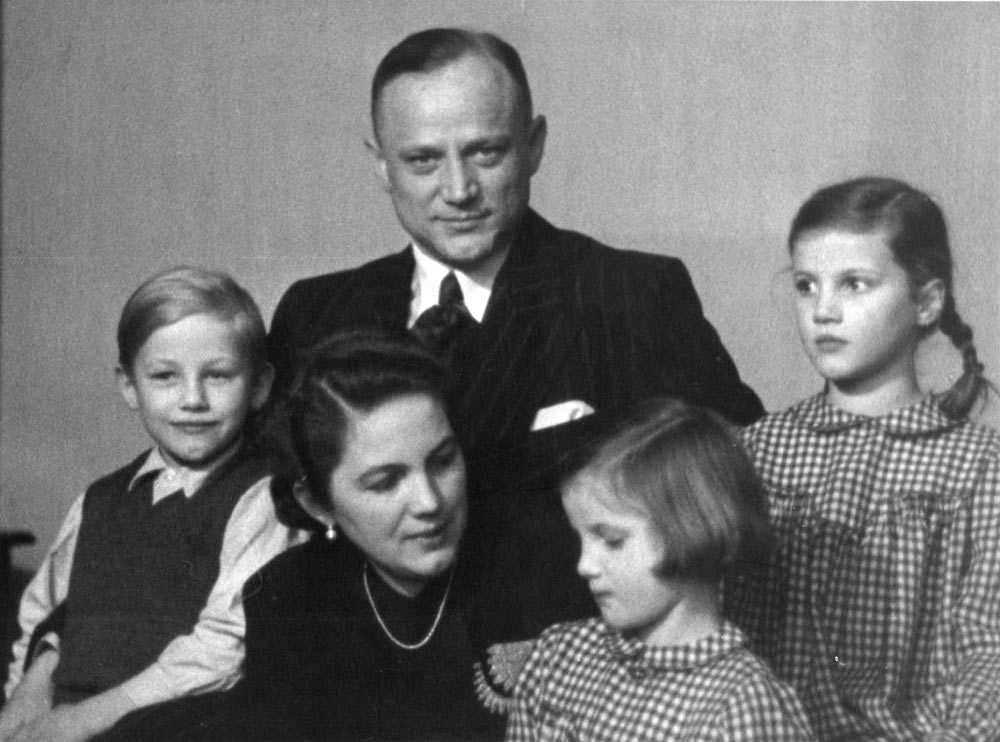
\includegraphics[width=6.588cm,height=4.888cm]{pictures/zulassungsarbeit-img034.jpg}

Dr. Karl Schlumprecht mit seiner Frau,
der Högn Tochter Frieda, und den Kindern Werner, Gertraud und Lilo\\
\end{supertabular}
\end{flushleft}
\end{minipage}
\end{center}
Högn wusste den guten Draht zu einem hohen NS-Funktionär zu nutzen –
nicht zum eigenen Vorteil, sondern zu dem der Allgemeinheit. Der
damalige Ruhmannsfeldener Bürgermeister Sturm stellte am 1. September
1938 an den Ministerialdirektor Schlumprecht im Finanzministerium einen
Antrag auf Unterstützung bei der Finanzierung des Außenputzes der
Ruhmannsfeldener Turnhalle. Der Vermerk auf dem Brief „In Abdruck an H.
Oberlehrer Högn, hier zur Kenntnis“ zeigt eindeutig, dass diese
Petition durch Högn, den ehemaligen Turnvereinsvorstand und
Veranstalter von Benefizkonzerten zugunsten der Errichtung der
Turnhalle, eingefädelt worden war. \footnote{Dokument Nr. 99, Brief von
Bürgermeister Sturm an Dr. Karl Schlumprecht, 1.9.1938}

Der Tatsache, dass Högn alle 12 Jahre des „1000-jährigen Reichs“
Schulleiter geblieben war, sagt zumindest aus, dass er den
Regimeführenden nicht negativ aufgefallen war. Seine Ernennung 1940 zum
Rektor der Volksschule zeigte, dass er zumindest auf der vorgegeben
Linie blieb. \footnote{Dokument Nr. 48, Zeitungsartikel aus Viechtacher
Bayerwald-Bote, 2.8.1958}

Eine Komposition mit eindeutig nationalsozialistischem Text lässt sicher
Rückschlüsse auf August Högns Gesinnung im 3. Reich zu. Auf den
Rückseiten der Notenblätter des Arrangements „Näher mein Gott zu dir!“
ist ein „Weihegesang“ zu finden. Auf jedem Notenblatt des Weihegesangs
steht „A. Högn“, wie bei allen August Högn eindeutig zugeordneten
Kompositionen. Högn hatte den Weihegesang nur durchgestrichen und das
Notenpapier weiter verwendet. Dieses Notenpapier war im Notenschrank
der Pfarrkirche St. Laurentius in Ruhmannsfelden aufzufinden. Hat
dieses der Komposition Högns zu Grunde liegende Gedicht – sein
Verfasser ist ungekannt – in der ersten Strophe noch Ähnlichkeit mit
Högns geistlicher Komposition, dem „Grablied für die auf dem Felde der
Ehre Gefallen op. 35“, so wird spätestens in der dritten Strophe klar,
wenn von „Steigt ein, der aus Walhallas Höhe, hoch ist es Zeit zur Tat“
die Rede ist und damit wohl die „Vorsehung“ Hitlers gemeint ist, dass
es sich nicht nur um einen patriotischen, sondern
nationalsozialistischen Text handelt. Der Weihegesang wurde mit
Sicherheit einige Male bei der weltlichen Trauerfeier für gefallene
Soldaten aufgeführt, die vor dem kirchlichem Requiem
stattfand, \footnote{Interview Nr. 6, Wilhelm Ederer, 2.1.2003, Absatz
6} da die mit Tinte geschriebenen Stimmen Flecken aufweisen, wie sie
nur Regentropfen verursachen können. Besonders irritiert, dass der
Weihegesang sowohl stilistisch als auch bezüglich der Besetzung, kaum
einen Unterschied zu den von Högn komponierten christlichen Grabliedern
ausmacht (siehe \ref{bkm:Ref100062461} „Weihegesang Es-Dur“, Seite
\pageref{bkm:Ref100062456}). Wie August Högn selbst zum Inhalt dieses
Texts stand, den er vertont hat, wird wohl unbekannt bleiben. Man kann
davon ausgehen, dass von der nationalsozialistischen Partei an ihn
Anfragen erfolgten, nicht nur die Gestaltung der geistlichen, sondern
auch der weltlichen Trauerfeier zu übernehmen. Wie er es in allen
anderen musikalischen Feldern gewohnt war, griff Högn auch hier zur
Feder, um passende Musik zu dem passenden Text zu schreiben. Doch
ernsthafte Konsequenzen wären sicher ausgeblieben, wenn er die Bitten
ausgeschlagen und schon gar nicht, wenn er ein Werk eines anderen
Komponisten aufgeführt hätte.

\begin{center}
\begin{minipage}{8.835cm}
\begin{center}
\tablefirsthead{}
\tablehead{}
\tabletail{}
\tablelasttail{}
\begin{supertabular}{m{8.635cm}}

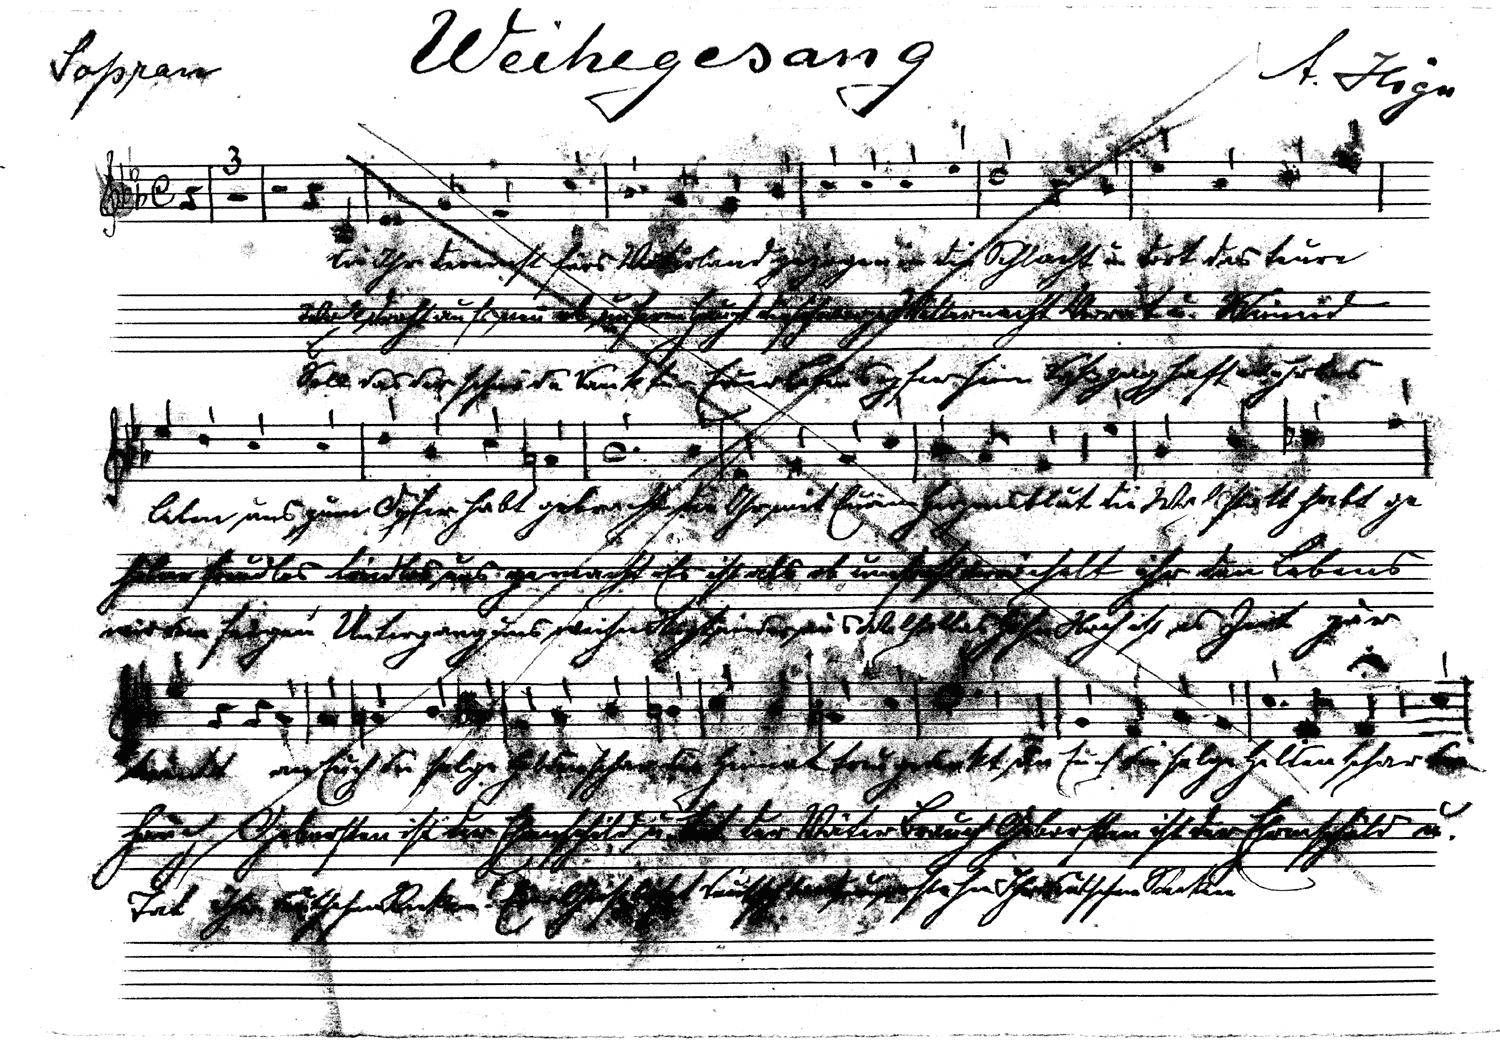
\includegraphics[width=8.453cm,height=5.678cm]{pictures/zulassungsarbeit-img035.png}

Sopran-Stimme des Weihegesang Es-Dur\\
\end{supertabular}
\end{center}
\end{minipage}
\end{center}
Als treuer Parteianhänger ist August Högn jedoch keinem der sechs zu
diesem Thema befragten Zeitzeugen in Erinnerung geblieben.\footnote{
Interview Nr. 4, Maria Schröck, 30.12.2002, Absatz 24; Interview Nr. 6,
Wilhelm Ederer, 2.1.2003, Absatz 24 – 26; Interview Nr. 16, Maria
Freisinger, 25.8.2004, Absatz 40; Interview Nr. 17, Max Holler,
26.8.2004, Absatz 18; Interview Nr. 24, Johann Glasschröder,
28.12.2004, Absatz 18; Interview Nr. 26, Eva Ertl, 9.2.2005, Absatz 28}
Als fanatische Anhängering der NS-Ideologie prägten sich einige der
Befragten stattdessen die seit 1942 \footnote{Reicheneder-Chronik,
Schulwesen, Blatt 112 Rückseite} an der Volksschule Ruhmannsfelden
unterrichtende Lehrerin Charlotte Werner ein. In ihrem Unterricht
musste Schüler aus einem Kalender Vorträge über herausragende
Persönlichkeiten des NS-Regimes halten. Vergleichbares ist aus Högns
Unterricht nicht bekannt. \footnote{Interview Nr. 6, Wilhelm Ederer,
2.1.2003, Absatz 24 – 28}

Rückschlüsse auf Högns Einstellung zu Hitlers Politik lassen sich nicht
zuletzt aus seinem in der Nachkriegszeit entstandenen Geschichtswerk
lesen. Folgende Textpassage aus der „Geschichte von Zachenberg“ lässt
sogar einen Interpretationsspielraum offen im Bezug auf seine anfangs
positive Einstellung zur NS-Ideologie, die sich im Lauf der Zeit hin
zur Ablehnung verändert haben könnte: \textit{„Die 1932/33
hereinbrechende Hitlerzeit hat zwar auf der einen Seite dieser
schlimmen Arbeitslosigkeit ein Ende gesetzt, aber auf der anderen Seite
den unheilvollen zweiten Weltkrieg heraufbeschworen, der das größte
Unglück, das je über ein Land und seine Bevölkerung kommen konnte, in
übervollem Maße über Deutschland ausgeschüttet hat.“ } \footnote{Högn,
Zachenberger, Blatt 17 (erster Teil)}\textit{ }Als ob er sich selbst
für seine anfängliche Gefolgschaft Hitlers rechtfertigen will, führt er
die Bekämpfung der Arbeitslosigkeit durch Hitler als eine zu würdigende
Errungenschaft an, geht aber sehr deutlich auf Distanz zur späteren
NS-Politik, die die „Kriegsfurie“, \footnote{Högn, Ruhmannsfelden,
Seite 16} – so nennt er den 2. Weltkrieg in der „Geschichte von
Ruhmannsfelden“ – verursacht hat, als er vollständig dessen Folgen
aufzählt. Wie ein Läuterungsversuch erscheinen die ausgedehnten
Passagen in seiner „Geschichte von Ruhmannsfelden,“ in denen er den
beiden Ruhmannsfeldener Widerständlern, Bürgermeister Sturm und
Studienrat Leonhard Donauer, die nur mit viel Glück der Exekution durch
die SS entronnen waren, ein Denkmal setzt. \footnote{Högn,
Ruhmannsfelden, Seite 32}

\begin{center}
\begin{minipage}{4.928cm}
\begin{flushleft}
\tablefirsthead{}
\tablehead{}
\tabletail{}
\tablelasttail{}
\begin{supertabular}{m{4.728cm}}

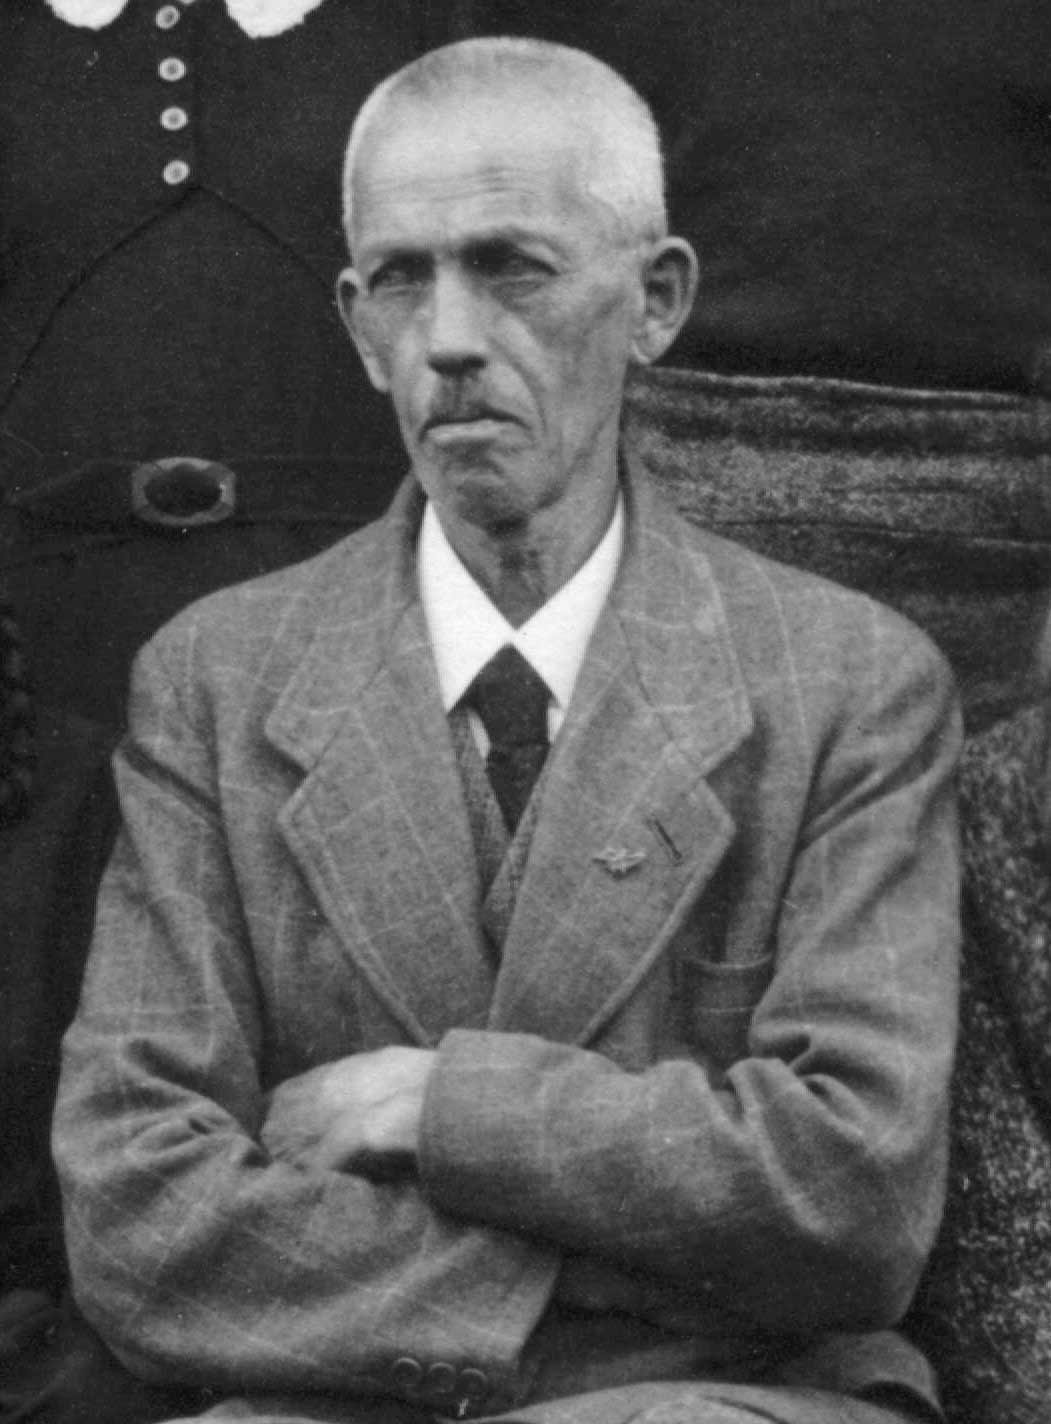
\includegraphics[width=4.503cm,height=6.103cm]{pictures/zulassungsarbeit-img036.jpg}

August Högn 1944: Das Bild eines eher
im inneren Konflikt lebenden, gebrochenen Mannes als das eines stolzen,
überzeugten Nazis.\\
\end{supertabular}
\end{flushleft}
\end{minipage}
\end{center}
Außer Frage steht, dass Högn kein Rassist war. Franz Danziger,
Kirchenchorsänger, Violinist und schließlich Högns Nachfolger als
Chorregent, war ein Halbjude, wie er im Jargon der Nationalsozialisten
geheißen hätte. Er erwähnte in seinen Memoiren über Högn kein einziges
schlechtes Wort. Viel mehr ehrte er seinen ehemaligen Lehrer, indem er
einige seiner Kompositionen aufführte.

Högns Chorregententätigkeit während des Krieges ist ebenfalls ein
Anhaltspunkt dafür, dass Högn nicht in allen Bereichen im Sinne der
NS-Ideologie gehandelt hat. Ein wirklich überzeugter Anhänger der
Weltanschauung Hitlers hätte versucht Religionen eher zu bekämpfen, als
sie durch Chorleiter- und Organistendienste doch maßgeblich zu fördern.
